% 图 27.1 —— **结构化重画**（2026-09-25，替换掉 `checks/emit_hand.py` 的逐段拟合稿）
%%
% 结构：一条数轴 + 左方括号 + 左圆括号 + 3 个实心点 + 一支凹背曲线箭头 + 4 个标签
%%
% 旧版是**描摹**：把每一段笔画单独拟合后发出来，连「箭头头」都被当成"一条很粗的短线"描
%   （图 81.5 上一度出现 `\draw[line width=7.0pt] (586,277)--(586,270);` 这种 7px 长的疙瘩），
%   渲染出来是黑疙瘩而不是箭头。本版改成**看懂结构后用 TikZ 画**。
%%
% 做法、约定、已踩过的坑 → `＜工作区＞\checks\redraw\README_重画流程.md`
% 本图圆/椭圆的中心与半径、标签的文字与位置，沿用 probe 的脚手架（那部分它是对的）。
%%
% ⚠ 本图 tikzpicture 是 y=-1pt（**y 翻转**）⇒ `arc` 的角向"递减"才是屏幕逆时针；
%   同一根线上的多段弧必须同向。改完务必拿原书并排、放大核箭头朝向。
%%
\documentclass[12pt]{standalone}
\usepackage{fontspec}
\setsansfont{Arial}
\newfontfamily\mfallback{DejaVu Sans}
\usepackage{tikz}
\usetikzlibrary{arrows.meta}
\begin{document}
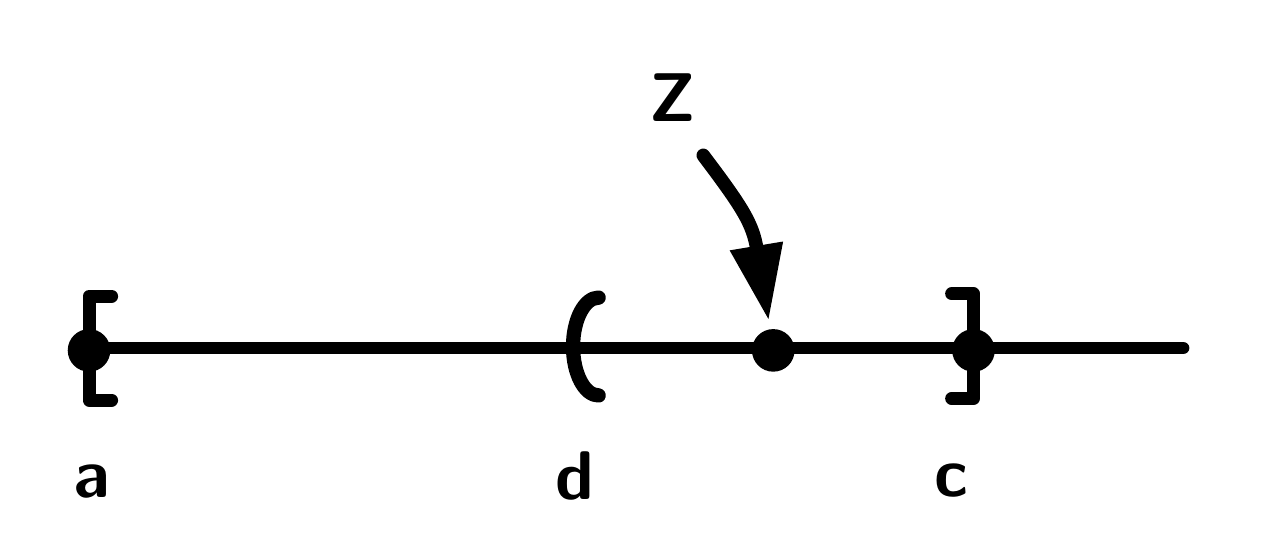
\begin{tikzpicture}[x=1pt, y=-1pt, line width=4.55pt, line cap=round, line join=round]

  % ── 数轴 ──
  \draw (22,115.76) -- (417.5,115.76);

  % ── a 处的方括号 [ （闭端点; 开口背向区间）──
  \draw[line width=4.7pt]
        (30.33,97.02) -- (22.17,97.02)
     -- (22.17,134.56) -- (30.33,134.56);

  % ── c 处的方括号 ] ──
  \draw[line width=4.7pt]
        (333.88,96.18) -- (341.77,96.18)
     -- (341.77,133.99) -- (333.88,133.99);

  % ── d 处的圆括号 ( ──
  \draw[line width=5.17pt]
        (206.32,97.54)
        .. controls (201.21,97.54) and (197.07,105.46) .. (197.07,115.22)
        .. controls (197.07,124.98) and (201.21,132.9) .. (206.32,132.9);

  % ── 三个实心点 a / z / c ──
  \foreach \p in {(22.17,116.61), (269.42,116.61), (341.77,116.61)}
     \fill \p circle (7.7);

  % ── 由 Z 指向 z 的弯箭头 ──
  % 2026-09-25: Stealth 的**默认 inset 不是 0**，会把头收窄 **28%**
        %   （实测：原书 17.8pt vs 我 13.9pt）。显式写 inset=0pt 后与 Triangle 等价。
        \draw[line width=4.9pt, -{Stealth[length=27.47pt, width=18.06pt, inset=0pt]}]
        (244.12,46.13) .. controls (258.49,65.18) and (261.99,70.84) .. (267.79,105.97);

  % ── 标签（anchor=base：直接钉在扫描量出的基线上）──
  \node[anchor=base,inner sep=0pt,font=\fontsize{24.5}{30.6}\selectfont] at (233.2,33.9) {\textsf{\textbf{\textit{Z}}}};
  \node[anchor=base,inner sep=0pt,font=\fontsize{30.2}{37.8}\selectfont] at (23.3,169.62) {\textsf{\textbf{\textit{a}}}};
  \node[anchor=base,inner sep=0pt,font=\fontsize{30.5}{38.1}\selectfont] at (197.7,170.43) {\textsf{\textbf{\textit{d}}}};
  \node[anchor=base,inner sep=0pt,font=\fontsize{30.0}{37.5}\selectfont] at (333.6,169.35) {\textsf{\textbf{\textit{c}}}};

  \path[use as bounding box] (0,0) rectangle (439,180);
\end{tikzpicture}
\end{document}
